\documentclass[12pt,letterpaper]{article}

\usepackage[T1]{fontenc}
\usepackage[utf8]{inputenc}
\usepackage[spanish,mexico,es-tabla,es-noshorthands]{babel}
\usepackage{newtxtext,newtxmath}          % Times New Roman
\usepackage[margin=2.5cm]{geometry}
\usepackage{graphicx}
\usepackage{float}
\usepackage{caption}
\usepackage{subcaption}
\usepackage{booktabs}
\usepackage{enumitem}
\usepackage{amsmath}          % no cargar amssymb: choca con \Bbbk de newtxmath
\usepackage{listings}
\usepackage{xcolor}
\usepackage{setspace}
\usepackage[colorlinks=true,allcolors=black]{hyperref}
\usepackage{todonotes}                    % usar [disable] para la versión final

\graphicspath{{evidencias/}{../assets/}}
\captionsetup{labelsep=colon,font=small,labelfont=bf}
\onehalfspacing
\setlength{\parskip}{6pt}

% Títulos de sección al estilo del formato de la profesora
\usepackage{titlesec}
\titleformat{\section}{\normalfont\large\bfseries}{}{0pt}{}
\titleformat{\subsection}{\normalfont\normalsize\bfseries}{}{0pt}{}

\definecolor{codekw}{RGB}{0,0,180}
\definecolor{codecm}{RGB}{0,128,0}
\definecolor{codestr}{RGB}{170,0,0}
\definecolor{codebg}{RGB}{248,248,248}

\lstdefinestyle{hdl}{
  language=VHDL,
  basicstyle=\ttfamily\footnotesize,
  keywordstyle=\color{codekw}\bfseries,
  commentstyle=\color{codecm}\itshape,
  stringstyle=\color{codestr},
  backgroundcolor=\color{codebg},
  numbers=left, numberstyle=\tiny\color{gray}, numbersep=8pt,
  frame=single, rulecolor=\color{gray!50},
  breaklines=true, breakatwhitespace=true,
  tabsize=2, showstringspaces=false, captionpos=b,
  extendedchars=true, inputencoding=utf8,
  literate={á}{{\'a}}1 {é}{{\'e}}1 {í}{{\'i}}1 {ó}{{\'o}}1 {ú}{{\'u}}1
           {Á}{{\'A}}1 {É}{{\'E}}1 {Í}{{\'I}}1 {Ó}{{\'O}}1 {Ú}{{\'U}}1
           {ñ}{{\~n}}1 {Ñ}{{\~N}}1 {ü}{{\"u}}1 {¿}{{?`}}1 {¡}{{!`}}1
}
\lstset{style=hdl}
% Para que el código comparta numeración con las figuras (en vez de tener su propio
% contador "Listing"), NO usar caption=/label= dentro de lstlisting/lstinputlisting.
% En su lugar, envolver el listado en un \begin{figure} normal y poner \caption y
% \label ahí (\figurename ya es "Figura" por babel-spanish):
%   \begin{figure}[H]
%     \centering
%     \lstinputlisting[style=hdl]{codigo/archivo.vhd}
%     \caption{Descripción del código.}
%     \label{fig:archivo}
%   \end{figure}


\begin{document}

\begin{titlepage}
\centering
\noindent
\begin{minipage}[c]{0.45\textwidth}\centering
  
\includegraphics[height=3.2cm]{logo-unam.jpg}
\end{minipage}\hfill
\begin{minipage}[c]{0.45\textwidth}\centering
  
\includegraphics[height=3.2cm]{logo-fi.png}
\end{minipage}

\vspace{1.2cm}
{\Large\bfseries UNIVERSIDAD NACIONAL AUTÓNOMA\\[2pt] DE MÉXICO\par}
\vspace{0.9cm}
{\large\bfseries FACULTAD DE INGENIERÍA\par}
\vspace{0.6cm}
{\large\bfseries INGENIERÍA EN COMPUTACIÓN\par}
\vspace{0.6cm}
{\bfseries Laboratorio de Organización de Arquitectura de Computadoras\par}
\vspace{0.9cm}
{\bfseries Reporte - Construcción de máquinas de Estados usando memorias: Direccionamiento Entrada-Estado\par}

\vspace{1.0cm}
\raggedright
{\bfseries NOMBRE DE LOS INTEGRANTES:}\\
Omar Alfonso Zendejas Labias \quad Grupo de Teoría: 04\\
Emiliano García Olvera \quad Grupo de Teoría: 02

\vspace{1.0cm}
{\bfseries NOMBRE DEL PROFESOR: ING. KAREN PÉREZ}

\vspace{0.6cm}
{\bfseries GRUPO: 06 \quad EQUIPO: 9}

\vspace{0.6cm}
{\bfseries SEMESTRE:} \underline{2027-1.}

\vspace{0.6cm}
\hfill {\bfseries FECHA DE ENTREGA: 22 de octubre de 2026}
\thispagestyle{empty}
\end{titlepage}

\setcounter{page}{1}

\section{Objetivo}

Construir una máquina de estados finita a partir de una carta ASM utilizando una memoria
como elemento central del diseño, ahora bajo el método de direccionamiento
entrada-estado. A diferencia del direccionamiento por trayectoria empleado en la
práctica anterior, aquí la dirección de memoria se forma únicamente con el estado
presente: la palabra almacenada indica cuál de las entradas debe sensarse y ofrece dos
estados siguientes y dos juegos de salidas, entre los cuales elige el valor de esa
entrada.

Para ello se diseñó una carta ASM de nueve estados, cuatro entradas y cuatro salidas
(dos con lógica estándar y dos con lógica negada), con salidas condicionales en varias
decisiones; se determinó el tamaño de memoria requerido, se obtuvo su contenido completo
y se implementó el sistema en VHDL sobre la tarjeta DE10-Lite mediante Quartus Prime,
verificando su funcionamiento por simulación y en hardware.

\section{Introducción}

Una carta ASM (\textit{Algorithmic State Machine}) representa gráficamente el
comportamiento de un circuito secuencial: los estados se dibujan como cajas
rectangulares, las condiciones de transición como cajas de decisión y las salidas que
dependen a la vez del estado y de las entradas como cajas ovaladas o salidas
condicionales. Estas últimas corresponden al modelo de Mealy, en el que las salidas
pueden cambiar sin que medie un flanco de \textit{clock}, a diferencia del modelo de
Moore, donde son función únicamente del estado presente \cite{mano}.

El método empleado en esta práctica, el \textbf{direccionamiento entrada-estado}, se
restringe a cartas ASM que sensan una sola entrada por estado \cite{savage}. Esa
restricción es justamente lo que permite reducir el tamaño de la memoria: mientras que en
el direccionamiento por trayectoria la dirección se formaba concatenando el estado
presente con \emph{todas} las variables de entrada, aquí la dirección se compone
exclusivamente del estado presente. La información sobre las entradas se traslada al
contenido de la palabra mediante un campo nuevo, la \textbf{parte de prueba}, que guarda
la representación binaria de la variable que debe sensarse en ese estado. Un selector de
entradas, implementado como un multiplexor, usa ese campo para elegir la señal
correspondiente.

En consecuencia, la palabra de memoria contiene dos estados siguientes en lugar de uno: la
\textbf{liga falsa}, que se toma cuando la entrada sensada vale cero, y la \textbf{liga
verdadera}, que se toma cuando vale uno. Un segundo multiplexor, el selector de liga,
escoge entre ambas según el valor entregado por el selector de entradas, y el resultado se
almacena en el registro de estado en el siguiente flanco de reloj.

Para manejar salidas condicionales, el diagrama de bloques básico debe modificarse
desdoblando también el campo de salidas en dos: el campo de \textbf{salidas falsas},
activo cuando la variable sensada vale cero, y el de \textbf{salidas verdaderas}, activo
cuando vale uno \cite{savage}. Un tercer multiplexor selecciona entre ellos con el mismo
criterio. Con esta estructura, el tamaño de la memoria queda determinado por

\begin{equation}
\text{Memoria} = 2^{n} \times m
\label{eq:tam}
\end{equation}

donde $n$ es el número de bits de dirección, que ahora equivale únicamente a los bits de
estado, y $m$ el número de bits por localidad, igual a la suma de los bits de prueba, de
liga falsa, de liga verdadera, de salidas falsas y de salidas verdaderas.

La ventaja frente al direccionamiento por trayectoria es que el número de localidades deja
de crecer exponencialmente con la cantidad de entradas: agregar una entrada más solo
ensancha el campo de prueba en lugar de duplicar la memoria. El precio es la restricción
de una sola prueba por estado, que obliga a desdoblar en estados auxiliares cualquier
estado que necesite evaluar dos condiciones.

\section{Desarrollo}

\subsection{Planteamiento: carta ASM}

Se diseñó la carta ASM de la figura \ref{fig:asm}, que cumple con las características
solicitadas: nueve estados, cuatro entradas ($Q_1$ a $Q_4$) y cuatro salidas, de las
cuales $S_1$ y $S_2$ operan con lógica estándar (activas en 1) y $S_3$ y $S_4$ con lógica
negada (activas en 0, lo que se indica con una barra sobre el nombre). La carta incluye
cuatro salidas condicionales, por encima de las tres que pide el manual, y respeta la
restricción del método: ningún estado sensa más de una entrada. El diseño preliminar a
mano se muestra en la figura \ref{fig:evid-asm}.

\begin{figure}[H]
  \centering
  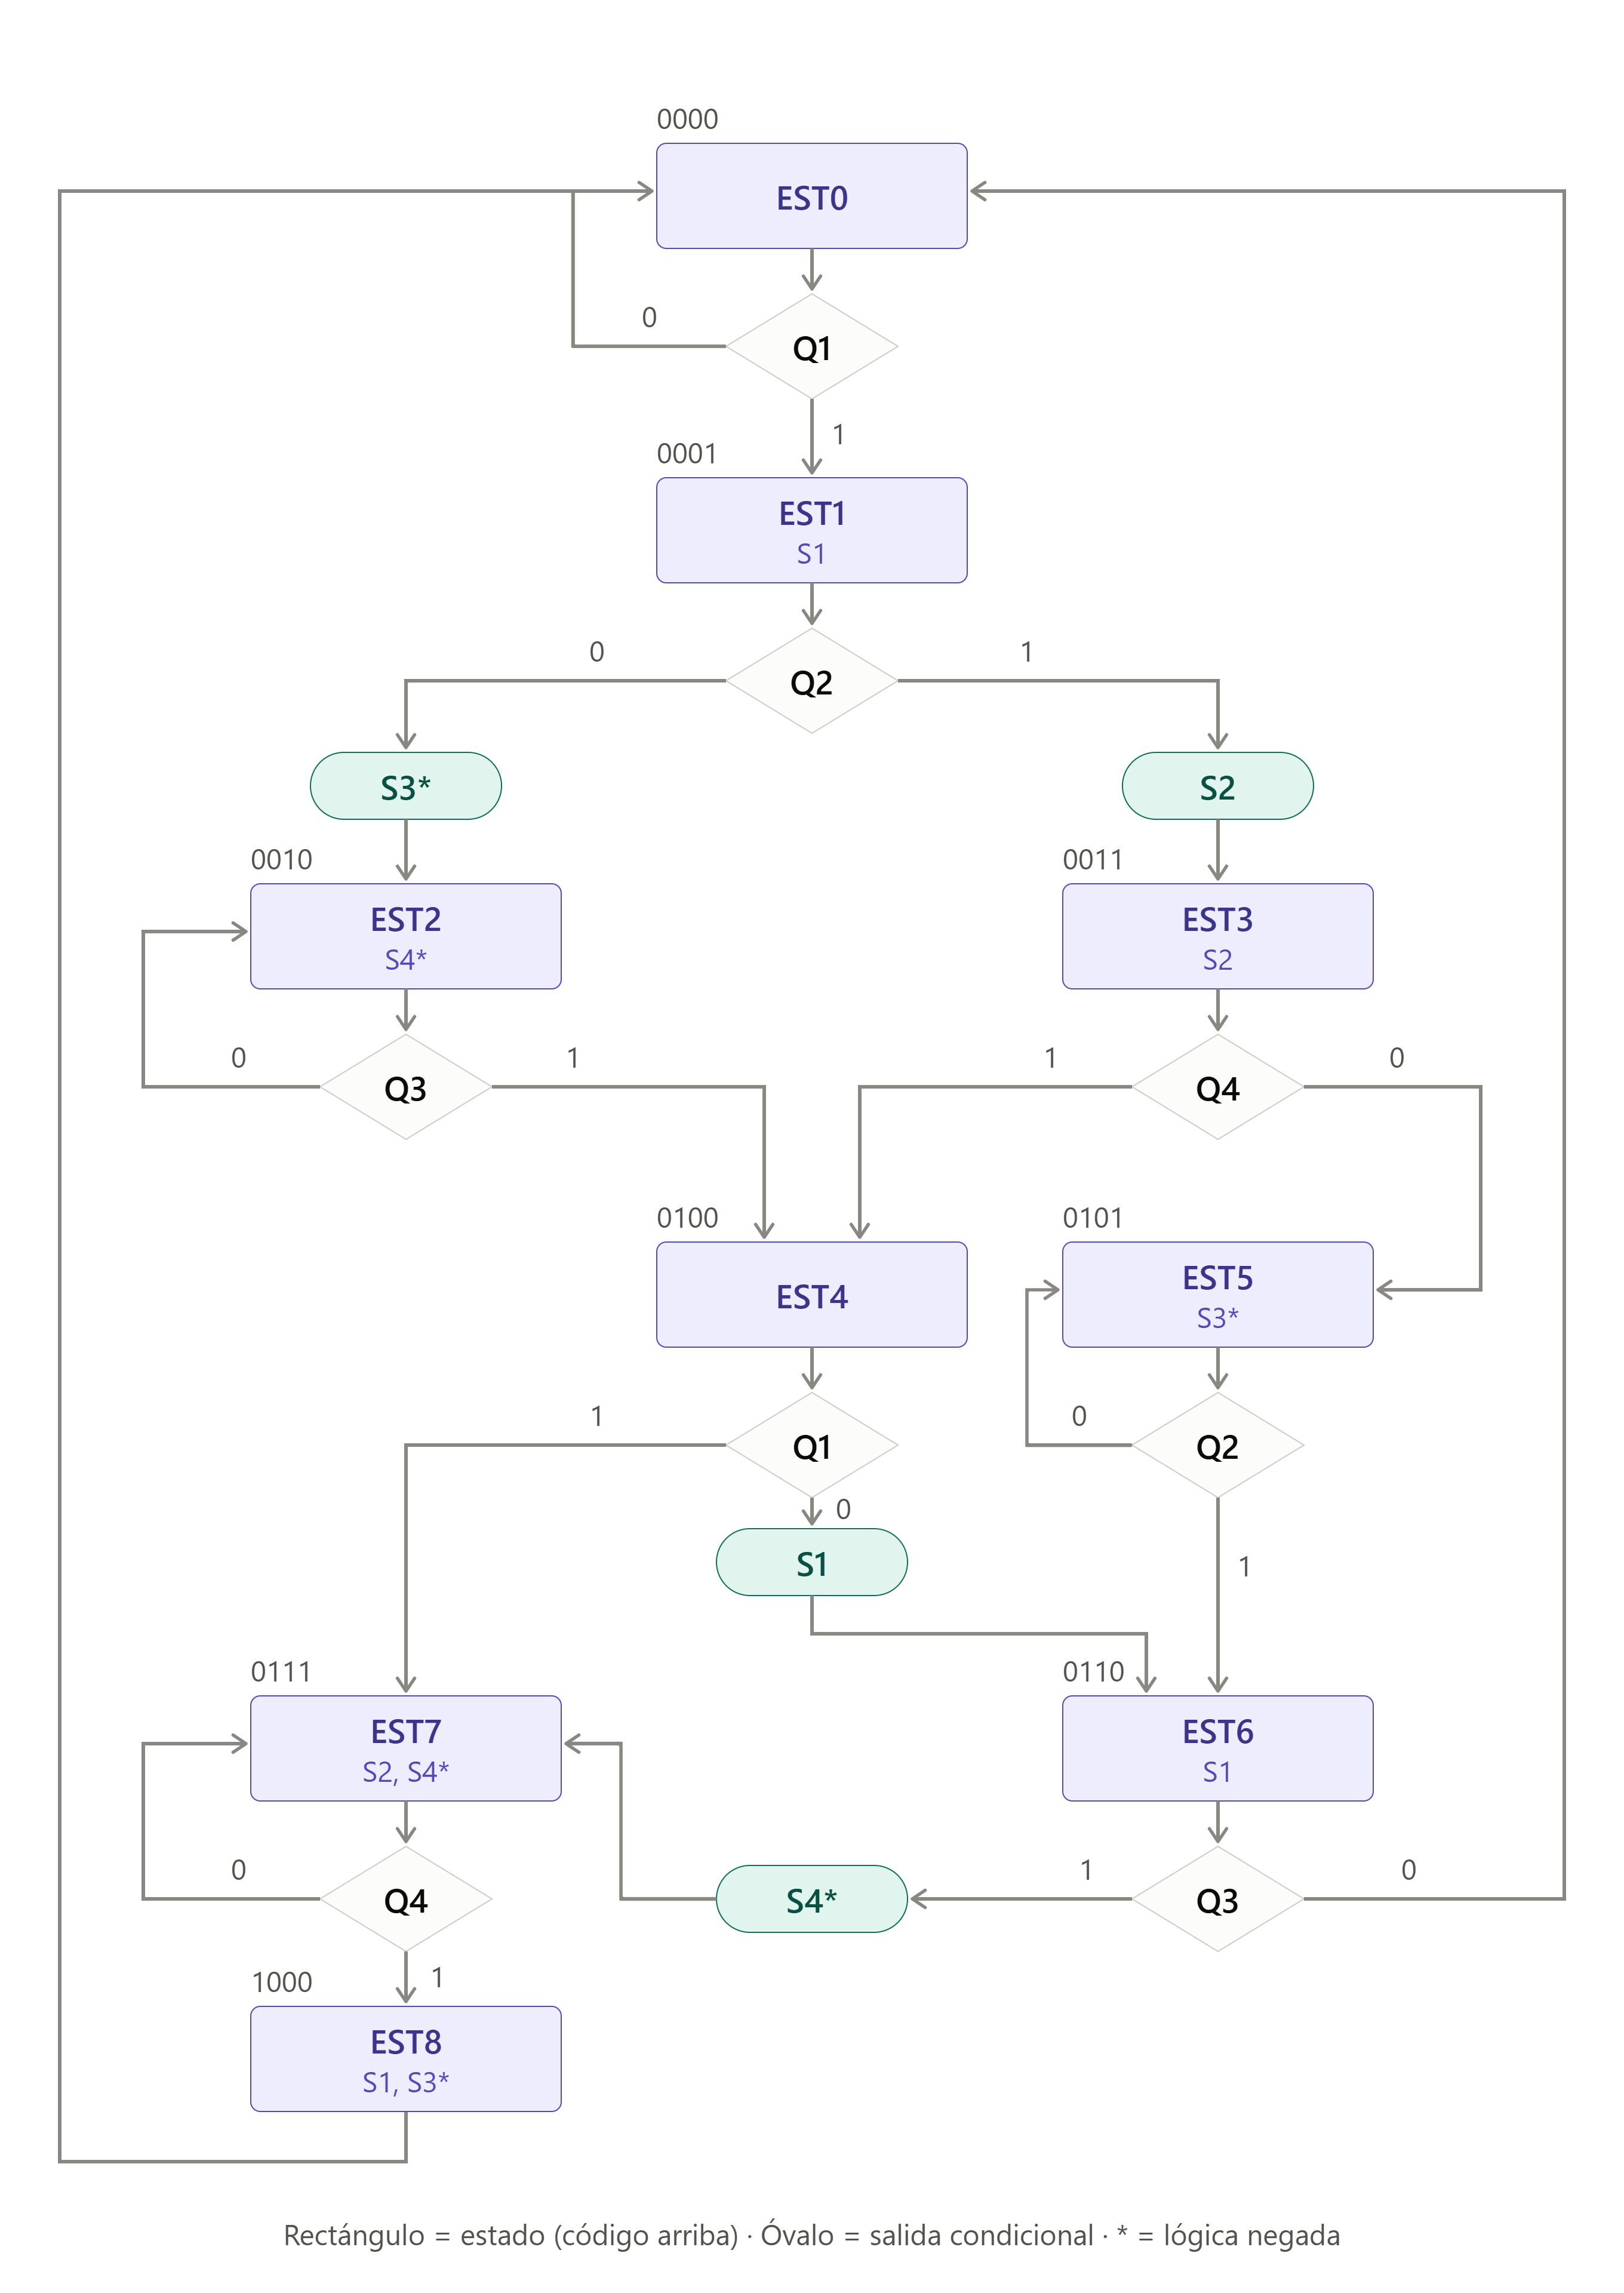
\includegraphics[width=0.78\textwidth]{practica4/evidencias/01-carta-asm.png}
  \caption{Carta ASM propuesta: nueve estados, cuatro entradas y cuatro salidas, con
  salidas condicionales en las decisiones de EST1, EST4 y EST6.}
  \label{fig:asm}
\end{figure}

\begin{figure}[H]
  \centering
  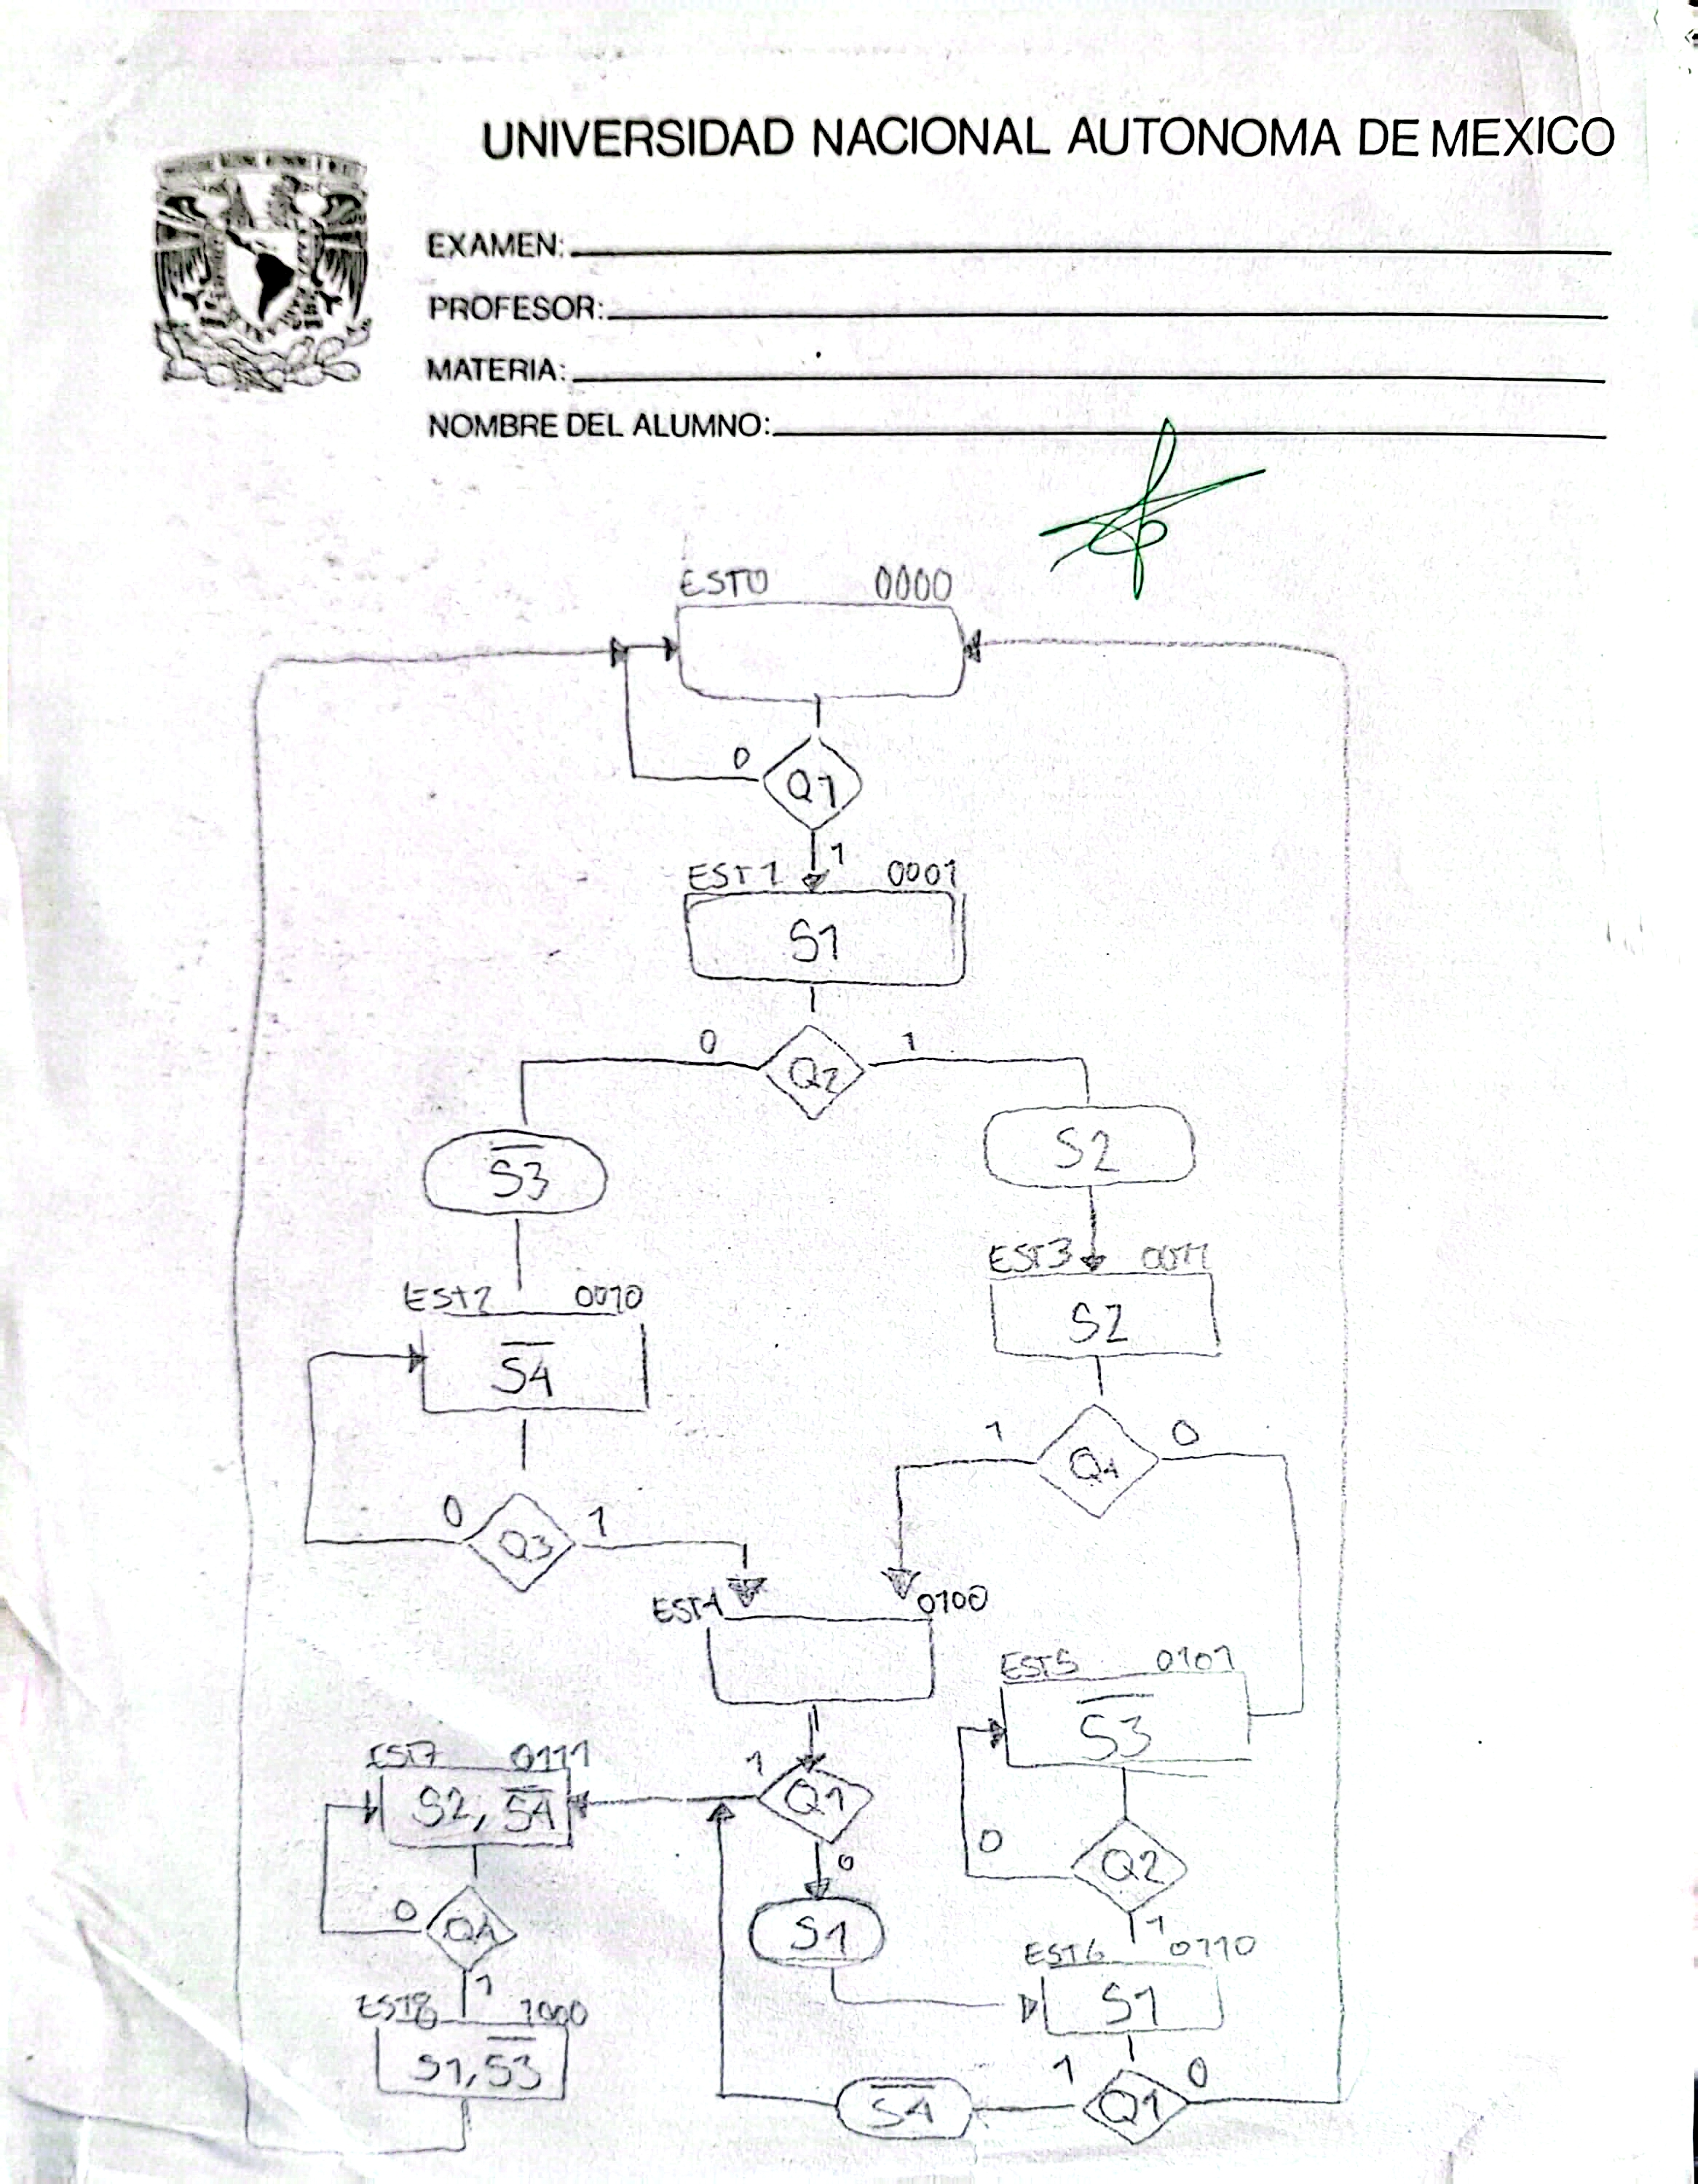
\includegraphics[width=0.9\textwidth,height=0.85\textheight,keepaspectratio]{practica4/evidencias/evidencia-carta-asm.jpg}
  \caption{Evidencia del diseño manual de la carta ASM previo a su captura digital, con la
  asignación de códigos de estado.}
  \label{fig:evid-asm}
\end{figure}

Antes de construir la tabla fue necesario asignar una representación binaria tanto a los
estados como a las entradas. Con nueve estados se requieren
$\lceil \log_2 9 \rceil = 4$ bits, de modo que el espacio de direcciones abarca 16
localidades y quedan siete códigos sin utilizar. Para las cuatro entradas bastan
$\lceil \log_2 4 \rceil = 2$ bits en el campo de prueba. Ambas asignaciones se resumen en
las tablas \ref{tab:estados} y \ref{tab:entradas}.

\noindent
\begin{minipage}[t]{0.56\textwidth}
\captionof{table}{Asignación binaria de los estados, con su salida incondicional y la
variable que sensan.}
\label{tab:estados}
\centering\small
\begin{tabular}{@{}l c l c@{}}
\toprule
\textbf{Estado} & \textbf{Código} & \textbf{Salida} & \textbf{Prueba} \\
\midrule
EST0 & \texttt{0000} & ---                     & $Q_1$ \\
EST1 & \texttt{0001} & $S_1$                   & $Q_2$ \\
EST2 & \texttt{0010} & $\overline{S_4}$        & $Q_3$ \\
EST3 & \texttt{0011} & $S_2$                   & $Q_4$ \\
EST4 & \texttt{0100} & ---                     & $Q_1$ \\
EST5 & \texttt{0101} & $\overline{S_3}$        & $Q_2$ \\
EST6 & \texttt{0110} & $S_1$                   & $Q_3$ \\
EST7 & \texttt{0111} & $S_2,\ \overline{S_4}$  & $Q_4$ \\
EST8 & \texttt{1000} & $S_1,\ \overline{S_3}$  & ---   \\
\bottomrule
\end{tabular}
\end{minipage}\hfill
\begin{minipage}[t]{0.40\textwidth}
\captionof{table}{Asignación binaria de las entradas en el campo de prueba.}
\label{tab:entradas}
\centering\small
\begin{tabular}{@{}c l@{}}
\toprule
\textbf{Prueba} & \textbf{Entrada} \\
\midrule
\texttt{00} & $Q_1$ \\
\texttt{01} & $Q_2$ \\
\texttt{10} & $Q_3$ \\
\texttt{11} & $Q_4$ \\
\bottomrule
\end{tabular}
\end{minipage}

\vspace{0.6cm}

El comportamiento de la máquina es el siguiente. EST0 no activa salidas y permanece en sí
mismo mientras $Q_1 = 0$; con $Q_1 = 1$ avanza a EST1. EST1 activa $S_1$ y sensa $Q_2$:
por la rama falsa activa además la salida condicional $\overline{S_3}$ y transita a EST2,
y por la verdadera activa $S_2$ y transita a EST3. EST2 activa $\overline{S_4}$ y se
autolaza mientras $Q_3 = 0$, avanzando a EST4 cuando $Q_3 = 1$. EST3 activa $S_2$ y, según
$Q_4$, va a EST5 (falsa) o a EST4 (verdadera). EST4 no activa salidas incondicionales y
sensa $Q_1$: con $Q_1 = 0$ activa la condicional $S_1$ y pasa a EST6, y con $Q_1 = 1$ pasa
a EST7. EST5 activa $\overline{S_3}$ y se autolaza mientras $Q_2 = 0$, avanzando a EST6
cuando $Q_2 = 1$. EST6 activa $S_1$ y sensa $Q_3$: con $Q_3 = 0$ regresa a EST0, y con
$Q_3 = 1$ activa además la condicional $\overline{S_4}$ y pasa a EST7. EST7 activa $S_2$ y
$\overline{S_4}$, se autolaza mientras $Q_4 = 0$ y avanza a EST8 cuando $Q_4 = 1$.
Finalmente, EST8 activa $S_1$ y $\overline{S_3}$ y, al no contener caja de decisión,
regresa incondicionalmente a EST0.

Respecto a la codificación de las salidas negadas se conservó el criterio de la práctica
anterior: almacenar en memoria el nivel físico de la señal, de modo que el bit de
$\overline{S_3}$ o $\overline{S_4}$ vale \texttt{0} cuando la salida está activa y
\texttt{1} cuando está en reposo. Así la palabra leída se conecta directamente a los pines
de salida sin inversores intermedios.

\subsection{Tamaño de la memoria necesaria}

Los cálculos manuales de la codificación y del tamaño se muestran en la figura
\ref{fig:evid-calc}. De acuerdo con la ecuación \ref{eq:tam}, la dirección se forma
únicamente con los 4 bits del estado presente, por lo que $n = 4$ y la memoria tiene
$2^4 = 16$ localidades. Cada localidad almacena los cinco campos del método:

\begin{figure}[H]
  \centering
  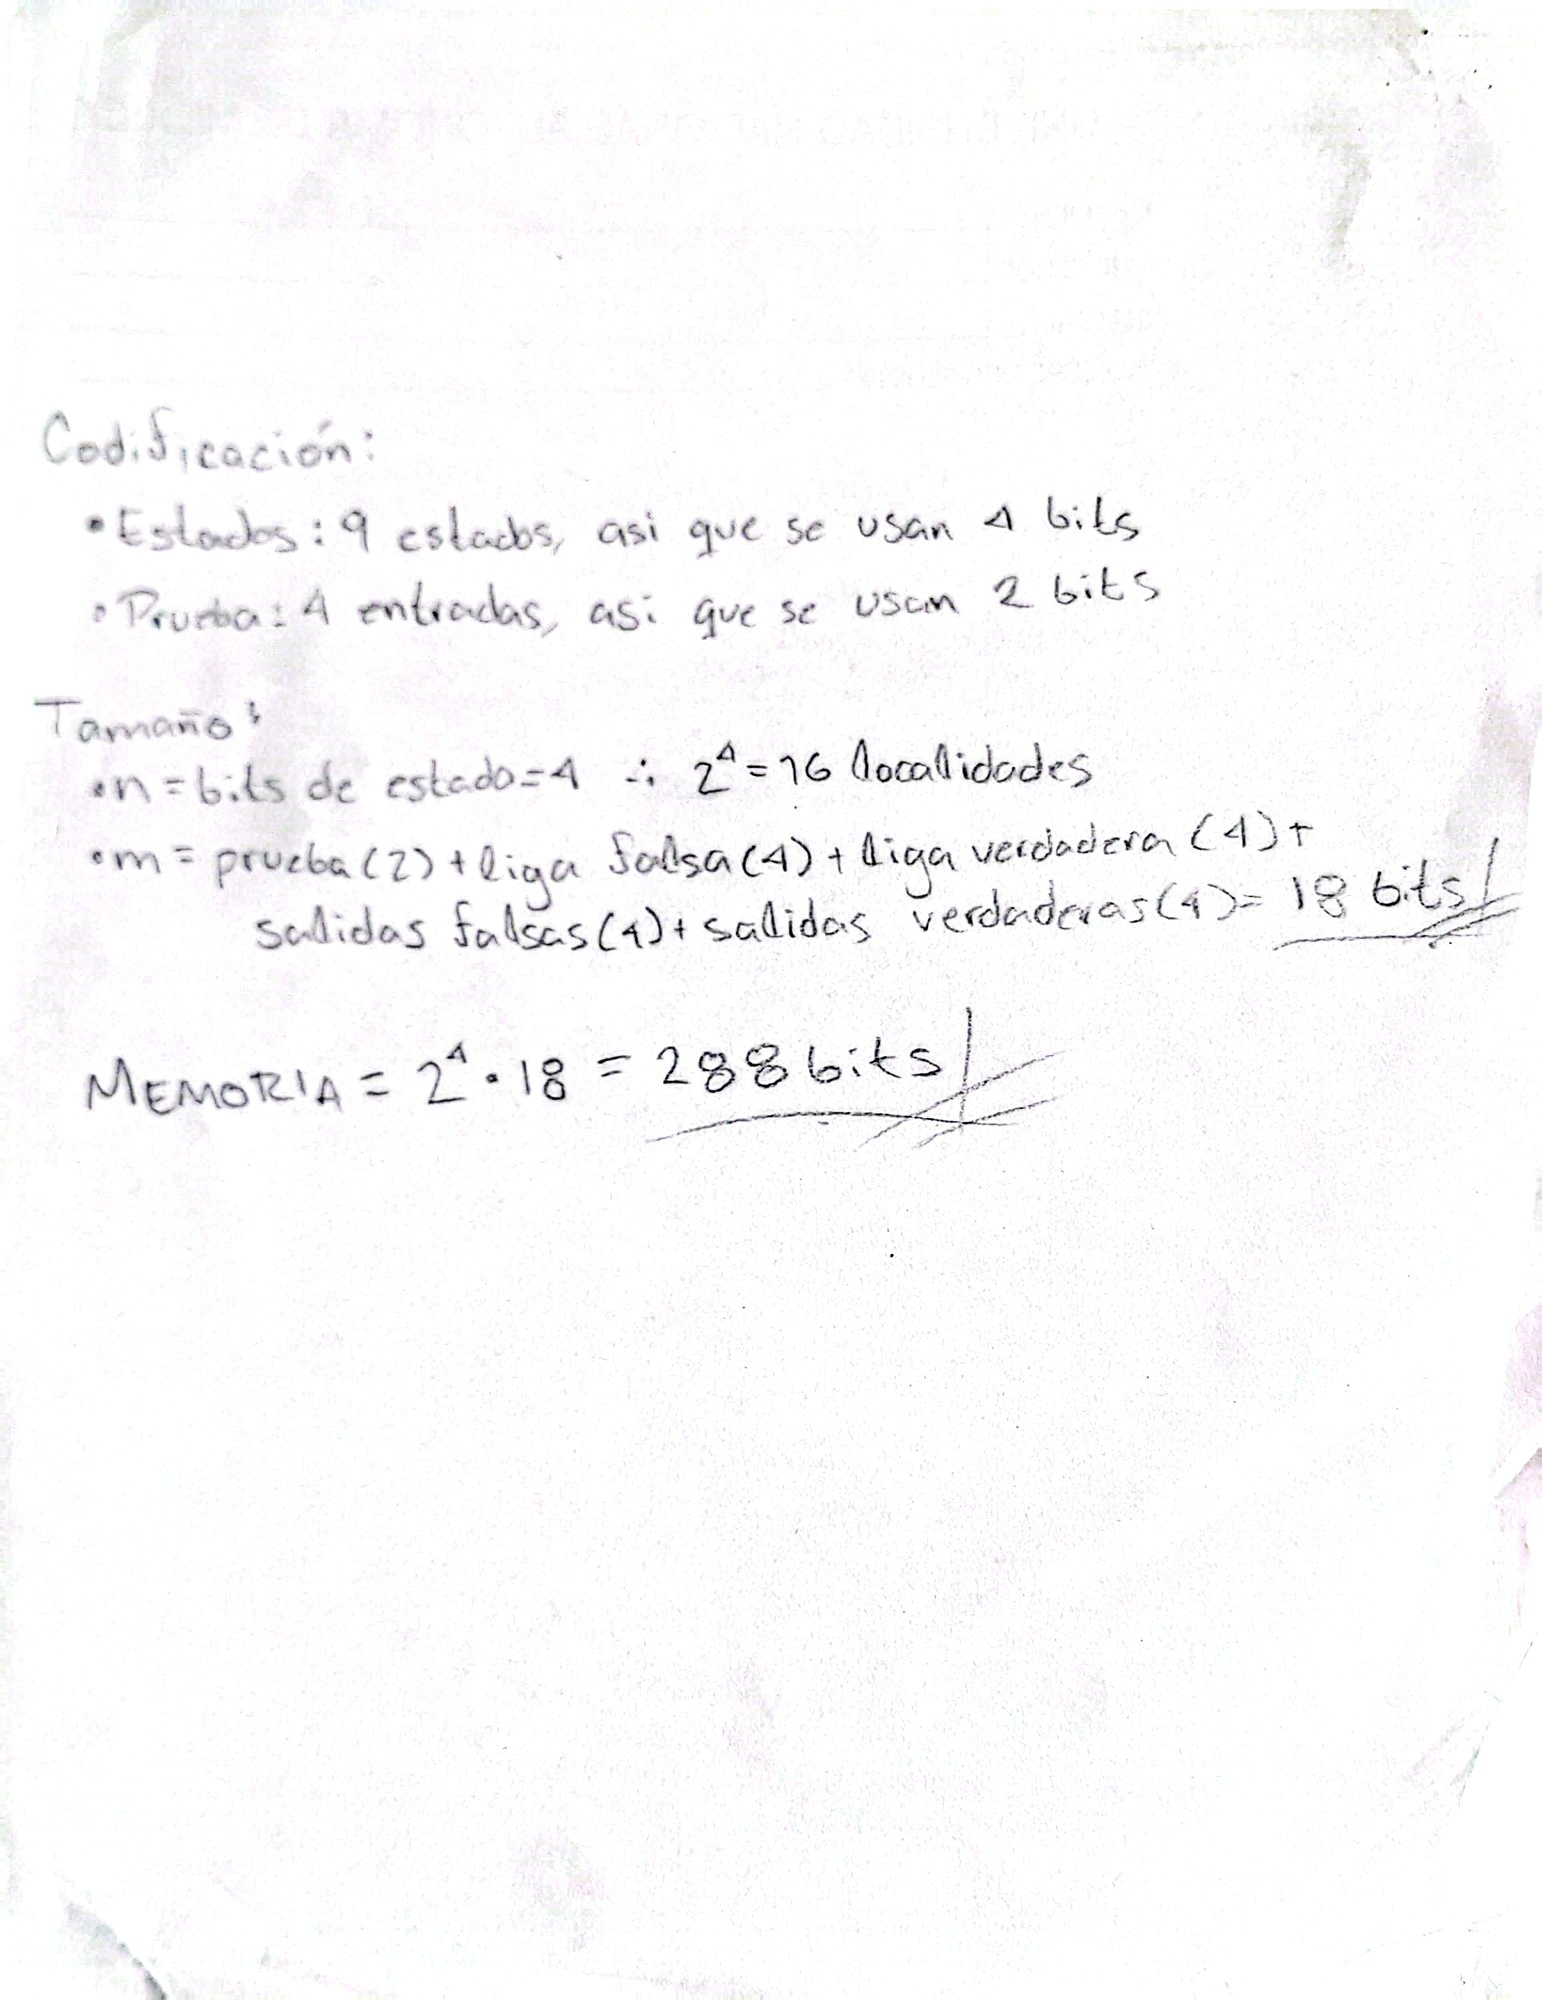
\includegraphics[width=0.9\textwidth,height=0.85\textheight,keepaspectratio]{practica4/evidencias/evidencia-calculos.jpg}
  \caption{Evidencia del cálculo manual de la codificación y del tamaño de la memoria: 4 bits
  de estado, 2 bits de prueba, 18 bits por localidad y 288 bits en total.}
  \label{fig:evid-calc}
\end{figure}

\begin{center}
\begin{tabular}{@{}l r@{}}
\toprule
\textbf{Campo} & \textbf{Bits} \\
\midrule
Parte de prueba (4 entradas) & 2 \\
Liga falsa (9 estados)       & 4 \\
Liga verdadera (9 estados)   & 4 \\
Salidas falsas               & 4 \\
Salidas verdaderas           & 4 \\
\midrule
\textbf{Total} $m$           & \textbf{18} \\
\bottomrule
\end{tabular}
\end{center}

Por lo tanto

\[
\text{Memoria} = 2^{4} \times 18 = 16 \times 18 = 288 \text{ bits},
\]

es decir, 16 localidades de 18 bits cada una. De ellas, nueve corresponden a estados que
existen en la carta ASM y las siete restantes (\texttt{1001} a \texttt{1111}) a códigos no
utilizados. Siguiendo la indicación del manual de considerar el llenado de todos los
estados representables con los bits asignados, a esas localidades se les dio un contenido
explícito de seguridad: ambas ligas apuntan a EST0 y los dos campos de salidas quedan en
reposo, de modo que si la máquina alcanzara uno de esos códigos por una condición anómala
retornaría al estado inicial en el siguiente flanco de reloj.

Conviene contrastar este resultado con el de la práctica anterior. Con direccionamiento
por trayectoria, una carta de nueve estados y cuatro entradas habría necesitado
$2^{4+4} = 256$ localidades; el direccionamiento entrada-estado las reduce a 16 a costa de
ensanchar cada palabra de 7 a 18 bits, lo que deja la memoria total en 288 bits frente a
los 1\,792 que habría exigido el método anterior.

\subsection{Contenido de la memoria}

El contenido se obtuvo recorriendo la carta ASM estado por estado. A diferencia de la
práctica anterior, no hay que enumerar las combinaciones de entrada: a cada estado le
corresponde una sola localidad, cuya dirección es su propio código. La palabra se organiza
como

\[
\text{dato} = \underbrace{\text{Prueba}}_{(17{:}16)} \ \Vert \
\underbrace{\text{Liga falsa}}_{(15{:}12)} \ \Vert \
\underbrace{\text{Liga verdadera}}_{(11{:}8)} \ \Vert \
\underbrace{\text{Salidas falsas}}_{(7{:}4)} \ \Vert \
\underbrace{\text{Salidas verdaderas}}_{(3{:}0)}
\]

En los estados cuya salida es incondicional, los campos de salidas falsas y verdaderas son
idénticos; sólo difieren en EST1, EST4 y EST6, que son los que tienen salidas
condicionales. En EST8 y en los estados no utilizados la parte de prueba es indiferente,
puesto que ambas ligas coinciden; se escribió \texttt{00} para dejar el campo en un valor
definido en lugar de un \emph{don't care}. La tabla \ref{tab:memoria} presenta las 16
localidades.

\begin{table}[htbp]
  \centering
  \caption{Contenido de memoria obtenido con direccionamiento entrada-estado. Las
  direcciones 9 a 15 corresponden a códigos de estado no utilizados: ambas ligas
  apuntan a EST0 y las salidas quedan en reposo.}
  \label{tab:memoria}
  \small
  \setlength{\tabcolsep}{6pt}
\begin{tabular}{@{}c c c c c c cccc cccc@{}}
\toprule
 & & \multicolumn{2}{c}{\textbf{Prueba}} & & & \multicolumn{4}{c}{\textbf{Salidas falsas}} & \multicolumn{4}{c}{\textbf{Salidas verdaderas}} \\
\cmidrule(lr){3-4} \cmidrule(lr){7-10} \cmidrule(lr){11-14}
\textbf{Dir.} & \textbf{Edo.} & bin & var & \textbf{LF} & \textbf{LV} & $S_1$ & $S_2$ & $\overline{S_3}$ & $\overline{S_4}$ & $S_1$ & $S_2$ & $\overline{S_3}$ & $\overline{S_4}$ \\
\midrule
0 & EST0 & \texttt{00} & $Q_1$ & \texttt{0000} & \texttt{0001} & \texttt{0} & \texttt{0} & \texttt{1} & \texttt{1} & \texttt{0} & \texttt{0} & \texttt{1} & \texttt{1} \\
1 & EST1 & \texttt{01} & $Q_2$ & \texttt{0010} & \texttt{0011} & \texttt{1} & \texttt{0} & \texttt{0} & \texttt{1} & \texttt{1} & \texttt{1} & \texttt{1} & \texttt{1} \\
2 & EST2 & \texttt{10} & $Q_3$ & \texttt{0010} & \texttt{0100} & \texttt{0} & \texttt{0} & \texttt{1} & \texttt{0} & \texttt{0} & \texttt{0} & \texttt{1} & \texttt{0} \\
3 & EST3 & \texttt{11} & $Q_4$ & \texttt{0101} & \texttt{0100} & \texttt{0} & \texttt{1} & \texttt{1} & \texttt{1} & \texttt{0} & \texttt{1} & \texttt{1} & \texttt{1} \\
4 & EST4 & \texttt{00} & $Q_1$ & \texttt{0110} & \texttt{0111} & \texttt{1} & \texttt{0} & \texttt{1} & \texttt{1} & \texttt{0} & \texttt{0} & \texttt{1} & \texttt{1} \\
5 & EST5 & \texttt{01} & $Q_2$ & \texttt{0101} & \texttt{0110} & \texttt{0} & \texttt{0} & \texttt{0} & \texttt{1} & \texttt{0} & \texttt{0} & \texttt{0} & \texttt{1} \\
6 & EST6 & \texttt{10} & $Q_3$ & \texttt{0000} & \texttt{0111} & \texttt{1} & \texttt{0} & \texttt{1} & \texttt{1} & \texttt{1} & \texttt{0} & \texttt{1} & \texttt{0} \\
7 & EST7 & \texttt{11} & $Q_4$ & \texttt{0111} & \texttt{1000} & \texttt{0} & \texttt{1} & \texttt{1} & \texttt{0} & \texttt{0} & \texttt{1} & \texttt{1} & \texttt{0} \\
8 & EST8 & \texttt{00} & --- & \texttt{0000} & \texttt{0000} & \texttt{1} & \texttt{0} & \texttt{0} & \texttt{1} & \texttt{1} & \texttt{0} & \texttt{0} & \texttt{1} \\
\midrule
\addlinespace[2pt]
9 & --- & \texttt{00} & --- & \texttt{0000} & \texttt{0000} & \texttt{0} & \texttt{0} & \texttt{1} & \texttt{1} & \texttt{0} & \texttt{0} & \texttt{1} & \texttt{1} \\
10 & --- & \texttt{00} & --- & \texttt{0000} & \texttt{0000} & \texttt{0} & \texttt{0} & \texttt{1} & \texttt{1} & \texttt{0} & \texttt{0} & \texttt{1} & \texttt{1} \\
11 & --- & \texttt{00} & --- & \texttt{0000} & \texttt{0000} & \texttt{0} & \texttt{0} & \texttt{1} & \texttt{1} & \texttt{0} & \texttt{0} & \texttt{1} & \texttt{1} \\
12 & --- & \texttt{00} & --- & \texttt{0000} & \texttt{0000} & \texttt{0} & \texttt{0} & \texttt{1} & \texttt{1} & \texttt{0} & \texttt{0} & \texttt{1} & \texttt{1} \\
13 & --- & \texttt{00} & --- & \texttt{0000} & \texttt{0000} & \texttt{0} & \texttt{0} & \texttt{1} & \texttt{1} & \texttt{0} & \texttt{0} & \texttt{1} & \texttt{1} \\
14 & --- & \texttt{00} & --- & \texttt{0000} & \texttt{0000} & \texttt{0} & \texttt{0} & \texttt{1} & \texttt{1} & \texttt{0} & \texttt{0} & \texttt{1} & \texttt{1} \\
15 & --- & \texttt{00} & --- & \texttt{0000} & \texttt{0000} & \texttt{0} & \texttt{0} & \texttt{1} & \texttt{1} & \texttt{0} & \texttt{0} & \texttt{1} & \texttt{1} \\
\bottomrule
\end{tabular}
\end{table}

\subsection{Implementación en VHDL y diagrama de bloques}

El sistema se describió en VHDL siguiendo el diagrama de bloques de la figura 3 del
manual, repartido en siete módulos. Los módulos se interconectaron en un diagrama de bloques
(archivo \texttt{.bdf}) de Quartus, que se configuró como entidad de nivel superior. La figura
\ref{fig:bdf} muestra esa interconexión. El lazo de datos es el siguiente: el registro de
estado entrega el estado presente, que direcciona la memoria; la palabra leída se separa en
sus cinco campos; el selector de entradas toma la parte de prueba y engancha una de las cuatro
entradas; y el valor de esa entrada gobierna simultáneamente al selector de liga, cuya salida
regresa al registro, y al selector de salidas, que maneja los pines $S_1$ a $S_4$. El estado
presente se expone hacia los LEDs para su observación.

\begin{figure}[H]
  \centering
  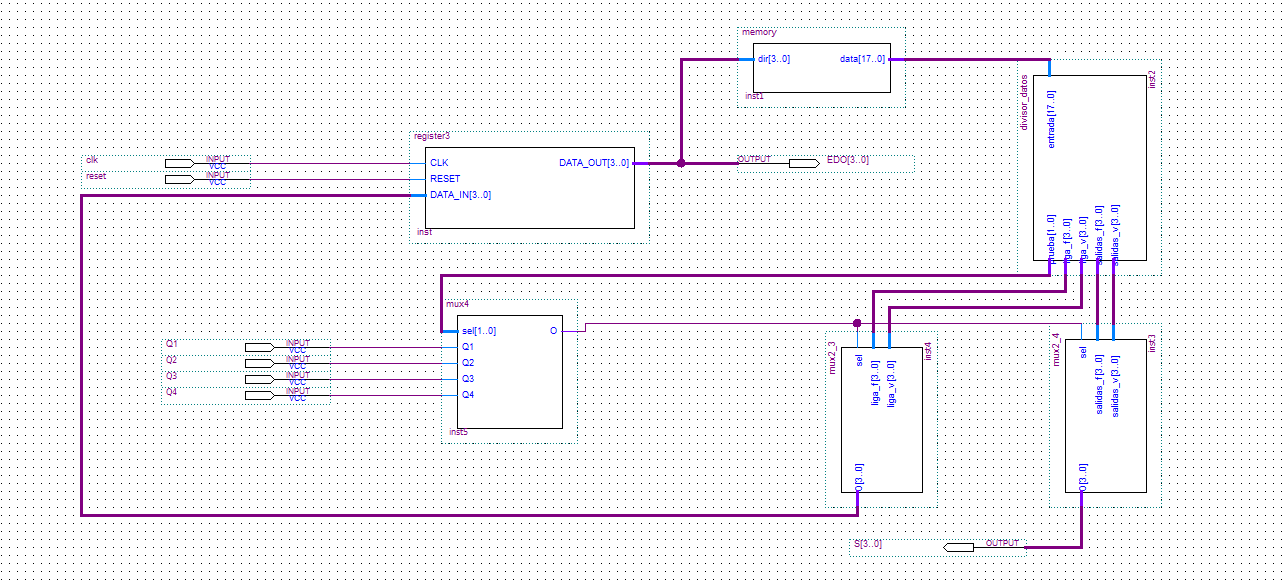
\includegraphics[width=\textwidth]{practica4/evidencias/diagrama-bloques.png}
  \caption{Diagrama a bloques de nivel superior (archivo \texttt{.bdf}) que interconecta la
  memoria, el divisor de datos, el registro de estado, el selector de entradas y los selectores
  de liga y de salidas.}
  \label{fig:bdf}
\end{figure}

El módulo \texttt{memory} implementa la ROM de 16 palabras de 18 bits. Cada asignación
corresponde a un renglón de la tabla \ref{tab:memoria} y está comentada con el estado y la
variable que sensa.

\lstinputlisting[style=hdl]{codigo/memory.vhd}
\captionof{figure}{Código VHDL de la memoria con las 16 localidades del direccionamiento
entrada-estado.}
\label{fig:memory}

El módulo \texttt{divisor\_datos} separa la palabra leída en los cinco campos del método.

\lstinputlisting[style=hdl]{codigo/divisor_datos.vhd}
\captionof{figure}{Código VHDL del divisor que separa la palabra en prueba, ligas y
salidas.}
\label{fig:divisor}

El selector de entradas, \texttt{mux4}, es el módulo que distingue a este método: toma los
dos bits de la parte de prueba y conecta a su salida únicamente la entrada indicada,
dejando las otras tres sin efecto sobre el comportamiento de la máquina en ese estado.

\lstinputlisting[style=hdl]{codigo/mux4.vhd}
\captionof{figure}{Código VHDL del selector de entradas gobernado por la parte de prueba.}
\label{fig:mux4}

Los dos multiplexores de 2 a 1 eligen, con el valor de la entrada sensada, entre liga
falsa y verdadera y entre salidas falsas y verdaderas.

\lstinputlisting[style=hdl]{codigo/mux2_3.vhd}
\captionof{figure}{Código VHDL del selector de liga.}
\label{fig:mux23}

\lstinputlisting[style=hdl]{codigo/mux2_4.vhd}
\captionof{figure}{Código VHDL del selector de salidas, que permite las salidas
condicionales.}
\label{fig:mux24}

El registro de estado es el único elemento secuencial del lazo. Tiene \textit{reset}
asíncrono activo en bajo que fuerza EST0 y, en cada flanco de subida, captura la liga
seleccionada. Se amplió a cuatro bits respecto al esqueleto original, como lo permite el
propio comentario del archivo, para alojar los nueve estados.

\lstinputlisting[style=hdl]{codigo/register3.vhd}
\captionof{figure}{Código VHDL del registro que almacena el estado presente.}
\label{fig:register}

Dado que el oscilador de la tarjeta opera a 50~MHz, las transiciones resultarían
imperceptibles. El divisor de frecuencia reinicia su contador al alcanzar
\texttt{X"2FAF080"} ($50\,000\,000$) y toma la salida del bit 25, lo que produce un periodo
de aproximadamente 1.0~s: una transición de estado por segundo.

\lstinputlisting[style=hdl]{codigo/div_frec.vhd}
\captionof{figure}{Código VHDL del divisor de frecuencia que fija la velocidad de la
máquina.}
\label{fig:divfrec}

\subsection{Asignación de pines}

Para la implementación en la tarjeta DE10-Lite (dispositivo MAX 10 10M50DAF484C7G) se
realizó la asignación de la tabla \ref{tab:pines}. Las cuatro entradas se asignaron a
interruptores deslizables, el \textit{reset} al botón \texttt{KEY0} (que la tarjeta entrega
en bajo al ser presionado, lo cual coincide con la polaridad del registro), las cuatro
salidas a \texttt{LEDR0}--\texttt{LEDR3} y los cuatro bits del estado presente a
\texttt{LEDR6}--\texttt{LEDR9}, ordenados de modo que el más significativo quede a la
izquierda.

\begin{table}[H]
  \centering
  \caption{Asignación de pines en la tarjeta DE10-Lite.}
  \label{tab:pines}
  \small
  \begin{tabular}{@{}l l l l@{}}
    \toprule
    \textbf{Señal} & \textbf{Pin} & \textbf{Recurso} & \textbf{Función} \\
    \midrule
    \texttt{CLK50}  & \texttt{PIN\_P11} & \texttt{MAX10\_CLK1\_50} & Reloj de 50 MHz \\
    \texttt{RESET}  & \texttt{PIN\_B8}  & \texttt{KEY0}   & \textit{Reset} activo en bajo \\
    \texttt{Q1}     & \texttt{PIN\_C10} & \texttt{SW0}    & Entrada $Q_1$ \\
    \texttt{Q2}     & \texttt{PIN\_C11} & \texttt{SW1}    & Entrada $Q_2$ \\
    \texttt{Q3}     & \texttt{PIN\_D12} & \texttt{SW2}    & Entrada $Q_3$ \\
    \texttt{Q4}     & \texttt{PIN\_C12} & \texttt{SW3}    & Entrada $Q_4$ \\
    \texttt{S1}     & \texttt{PIN\_A8}  & \texttt{LEDR0}  & Salida $S_1$ (activa en 1) \\
    \texttt{S2}     & \texttt{PIN\_A9}  & \texttt{LEDR1}  & Salida $S_2$ (activa en 1) \\
    \texttt{S3}     & \texttt{PIN\_A10} & \texttt{LEDR2}  & Salida $\overline{S_3}$ (activa en 0) \\
    \texttt{S4}     & \texttt{PIN\_B10} & \texttt{LEDR3}  & Salida $\overline{S_4}$ (activa en 0) \\
    \texttt{EDO[3]} & \texttt{PIN\_B11} & \texttt{LEDR9}  & Bit 3 del estado presente \\
    \texttt{EDO[2]} & \texttt{PIN\_A11} & \texttt{LEDR8}  & Bit 2 del estado presente \\
    \texttt{EDO[1]} & \texttt{PIN\_D14} & \texttt{LEDR7}  & Bit 1 del estado presente \\
    \texttt{EDO[0]} & \texttt{PIN\_E14} & \texttt{LEDR6}  & Bit 0 del estado presente \\
    \bottomrule
  \end{tabular}
\end{table}

\section{Análisis de resultados}

El proyecto se compiló en Quartus Prime 25.1std Lite Edition sin errores. La tabla
\ref{tab:sintesis} resume los recursos utilizados y el desempeño reportado.

\begin{table}[H]
  \centering
  \caption{Resumen de compilación del proyecto en Quartus Prime 25.1std.}
  \label{tab:sintesis}
  \begin{tabular}{@{}l r@{}}
    \toprule
    \textbf{Parámetro} & \textbf{Valor} \\
    \midrule
    Elementos lógicos            & 71 / 49\,760 ($<1\%$) \\
    Registros dedicados          & 32 / 49\,760 ($<1\%$) \\
    Pines de E/S                 & 14 / 360 (4\%) \\
    Bits de memoria embebida     & 0 / 1\,677\,312 (0\%) \\
    $F_{max}$ (modelo 1200 mV, 85 $^\circ$C) & 189.68 MHz \\
    Errores de compilación       & 0 \\
    \bottomrule
  \end{tabular}
\end{table}

Dos cifras de la tabla \ref{tab:sintesis} merecen comentario. La primera es el conteo de 32
registros, que coincide con lo esperado: 28 corresponden al contador del divisor de
frecuencia y los 4 restantes al registro de estado, lo que confirma que el único elemento
secuencial del lazo de la máquina es ese registro. La segunda es que la herramienta reporta
cero bits de memoria embebida: la ROM de 288 bits no se mapeó a los bloques M9K del
dispositivo sino que se sintetizó como lógica combinacional dentro de los 71 elementos
lógicos, lo cual es razonable dado su tamaño y no altera el comportamiento del circuito.
Los 189.68~MHz de frecuencia máxima superan ampliamente los 50~MHz del oscilador, de modo
que el diseño opera con holgura; la advertencia de incumplimiento temporal que emite el
analizador se debe únicamente a que el proyecto no incluye un archivo \texttt{.sdc}, y en
ausencia de restricciones Quartus asume un requisito por omisión de 1~GHz.

\subsection{Simulación funcional}

Antes de programar la tarjeta se verificó el diseño mediante simulación funcional con
un \textit{testbench} autoverificable. El banco de pruebas aplica una secuencia de 22
vectores de entrada que recorre los nueve estados y ambas ramas de cada decisión, incluidas
las cuatro salidas condicionales y el paso EST7 $\rightarrow$ EST8 $\rightarrow$ EST0. En cada
transición compara el estado resultante con el previsto por la carta ASM mediante sentencias
\texttt{assert}, y al finalizar reporta que las 22 transiciones coinciden con la carta. La
simulación concluyó sin discrepancias.

La simulación se compiló y ejecutó con GHDL, y la forma de onda se visualizó con GTKWave a
partir del archivo \texttt{sim.vcd}. El \textit{testbench} instancia la cadena funcional
completa (memoria, divisor de datos, selector de entradas, los dos multiplexores de 2 a 1 y
el registro de estado) manejando el registro con un reloj directo de 10~ns. Se omite
deliberadamente el divisor de frecuencia, ya que ese módulo sólo fija la velocidad perceptible
en la tarjeta y simularlo exigiría $2^{25}$ ciclos por cada flanco.

\begin{figure}[H]
  \centering
  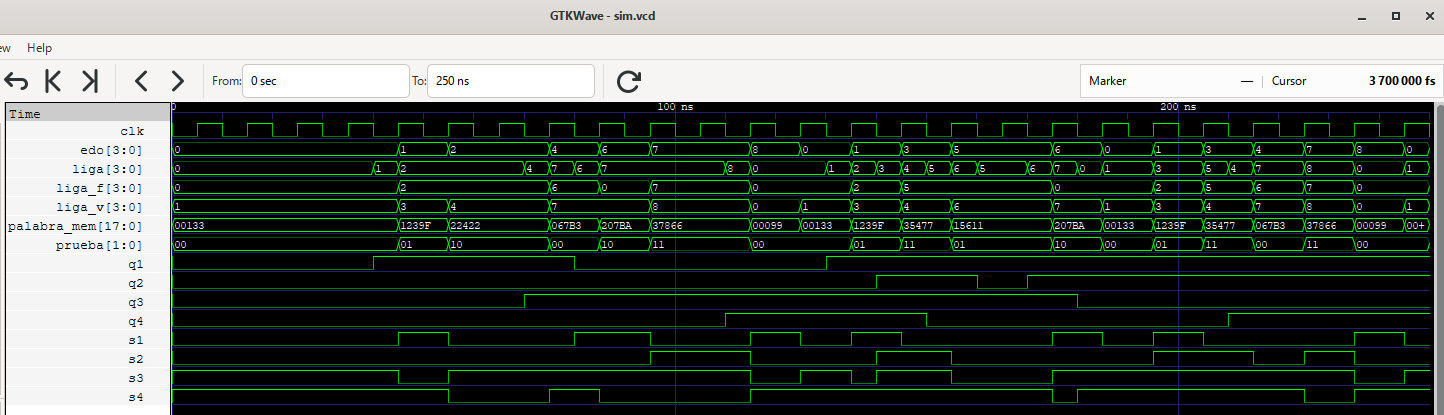
\includegraphics[width=\textwidth]{practica4/evidencias/simulacion.png}
  \caption{Forma de onda de la simulación funcional. Se muestran el reloj, el estado presente
  (\texttt{edo}), la liga seleccionada y sus versiones falsa y verdadera, la palabra leída de
  memoria (\texttt{palabra\_mem}), la parte de prueba, las entradas $Q_1$ a $Q_4$ y las
  salidas $S_1$ a $S_4$, durante las 22 transiciones (0 a 250~ns).}
  \label{fig:sim}
\end{figure}

En la figura se observa que el estado presente recorre los nueve estados de la carta y regresa
a EST0 al final del recorrido. Cada cambio de estado coincide con un flanco de reloj, y las
salidas $S_1$ a $S_4$ se activan según la rama tomada en cada decisión.

\subsection{Verificación en la tarjeta}

Durante la sesión de laboratorio se programó la DE10-Lite con el diseño y se observó su
comportamiento. Con los cuatro interruptores en bajo, la máquina permanece en EST0. Esto es
consistente con la liga falsa de la dirección 0, que apunta a sí misma mientras $Q_1 = 0$.

Al activar $Q_1$, $Q_2 = 0$, $Q_3 = 1$ y $Q_4 = 1$, la máquina recorre el lazo
EST0$\to$EST1$\to$EST2$\to$EST4$\to$EST7$\to$EST8$\to$EST0. Cada transición corresponde a
una liga de la tabla \ref{tab:memoria}: EST1 toma la liga falsa porque $Q_2 = 0$, EST2 toma
la liga verdadera porque $Q_3 = 1$, EST4 toma la liga verdadera porque $Q_1 = 1$, EST7 toma
la liga verdadera porque $Q_4 = 1$, y EST8 regresa a EST0 de forma incondicional.

Al detenerse en un estado que se autolaza (EST2, EST5 o EST7), los interruptores que no
corresponden a su parte de prueba no producen ningún efecto. Esto muestra que el selector de
entradas sensa únicamente la variable indicada por la palabra almacenada, y es la diferencia
principal con el direccionamiento por trayectoria.

Por último, \texttt{LEDR2} y \texttt{LEDR3} permanecen encendidos en reposo, ya que la salida
negada almacena un \texttt{1} cuando está inactiva. Se apagan al activarse $\overline{S_3}$ o
$\overline{S_4}$, en los estados donde la carta ASM las activa.

\section{Conclusiones individuales}

\subsection{Omar Alfonso Zendejas Labias}

Se cumplió el objetivo de la práctica. La máquina de nueve estados quedó implementada con
una memoria de 16 localidades de 18 bits y funcionó tanto en simulación como en la tarjeta
siguiendo la carta ASM. Lo que más me sirvió fue comparar este método con el de la práctica
anterior: aquí la dirección es nada más el estado presente, y por eso la memoria baja de
las 256 localidades que habría pedido el direccionamiento por trayectoria a solo 16, aunque
cada palabra pase de 7 a 18 bits. En la tarjeta eso se nota de inmediato, porque estando en
un estado que se autolaza los interruptores que no corresponden a su parte de prueba no
hacen absolutamente nada; ahí se entiende para qué sirve el selector de entradas. También
me quedó claro por qué el método exige una sola prueba por estado, ya que la palabra solo
tiene espacio para dos ligas.

\subsection{Emiliano García Olvera}

Considero que se cumplió el objetivo de la práctica. Con el direccionamiento entrada-estado
se construyó una máquina de nueve estados a partir de la carta ASM, usando una memoria de
16 localidades de 18 bits (tabla \ref{tab:memoria}), lo que da un total de 288 bits. Frente
al direccionamiento por trayectoria, que habría requerido 256 localidades y 1\,792 bits, la
reducción es considerable. La tabla \ref{tab:sintesis} muestra que el diseño compila sin
errores, utiliza menos del 1\% de los elementos lógicos del dispositivo y alcanza una
frecuencia máxima de 189.68~MHz, por encima de los 50~MHz del oscilador. La simulación
funcional con la secuencia de 22 vectores no presentó discrepancias, lo que confirma que
cada transición coincide con la carta ASM. Lo que más me aportó la práctica fue entender por
qué este método exige una sola prueba por estado: la palabra sólo tiene espacio para dos
ligas, y ese límite es el costo que se paga por reducir el tamaño de la memoria.

\renewcommand{\refname}{Bibliografía}
\begin{thebibliography}{9}
\bibitem{savage} J. Savage Carmona, G. Vázquez y N. E. Chávez Rodríguez,
  \emph{Diseño de microprocesadores}. Ciudad de México, México: Facultad de Ingeniería,
  Universidad Nacional Autónoma de México, 2017. [En línea]. Disponible:
  \url{http://profesores.fi-b.unam.mx/luist/archivos/MicroprocesadoresSavage.pdf}
\bibitem{mano} M. M. Mano y M. D. Ciletti, \emph{Diseño digital}, 5a ed.
  Naucalpan de Juárez, México: Pearson Educación, 2013.
\end{thebibliography}

\end{document}
